\documentclass[11pt]{article}
\usepackage[english]{babel}
\usepackage{minted}
\usepackage{amsmath}
\usepackage{amsthm}
\usepackage{graphicx}
\usepackage{subcaption}
\usepackage{booktabs}
\usepackage[left=25mm, top=25mm, bottom=30mm, right=25mm]{geometry}
\usepackage[colorlinks=true, linkcolor=blue, urlcolor=cyan]{hyperref}

\title{COL774\\Assignment 1}
\author{Sayam Sethi}
\date{12 September 2021}

\renewcommand\thesubsection{\thesection.\alph{subsection}}

\begin{document}

\maketitle

\tableofcontents

\section{Linear Regression}

\subsection{Batch Gradient Descent}
On performing \textit{batch gradient descent} with $\eta=0.05$ and $\varepsilon=10^{-15}$ (difference between consecutive cost functions), we learn the following model (rounded off to $5$ decimal places):
\begin{equation}
    \theta=
    \begin{pmatrix}
        0.99662\\
        0.00134
    \end{pmatrix}
\end{equation}
The learning takes $309$ iterations.

\subsection{Regression Plot}
\begin{figure}[H]
    \centering
    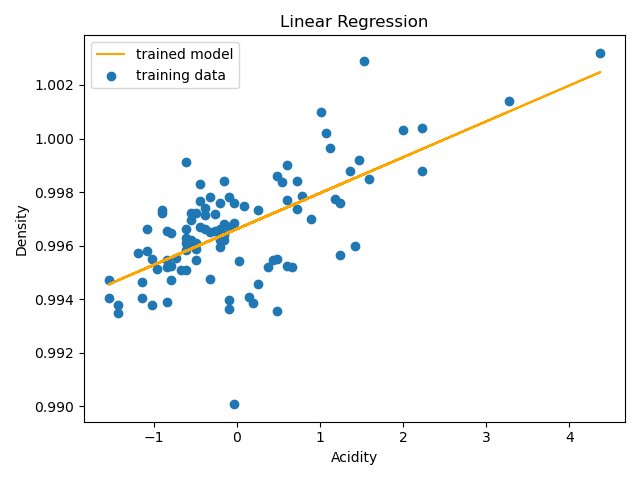
\includegraphics[width=0.6\textwidth]{Q1/output/b.png}
    \caption{Data and Hypothesis plot for Q1}
\end{figure}

\subsection{3D Mesh and Learning $\theta$}
\begin{figure}[H]
    \centering
    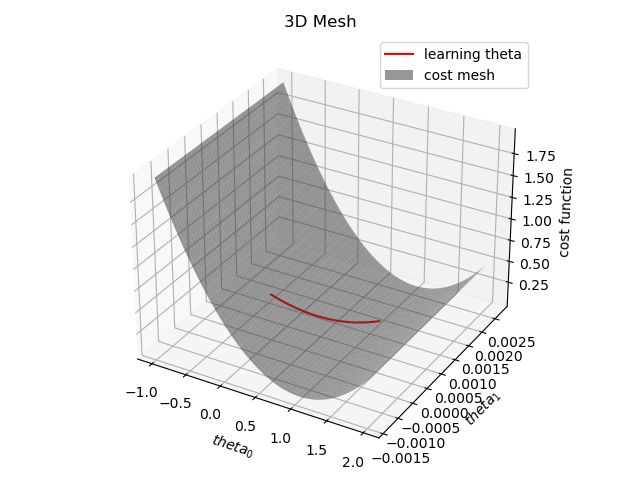
\includegraphics[width=0.7\textwidth]{Q1/output/c.png}
    \caption{Mesh of Cost Function and Movement of $\theta$}
\end{figure}

\subsection{Learning over the Contour}
\begin{figure}[H]
    \centering
    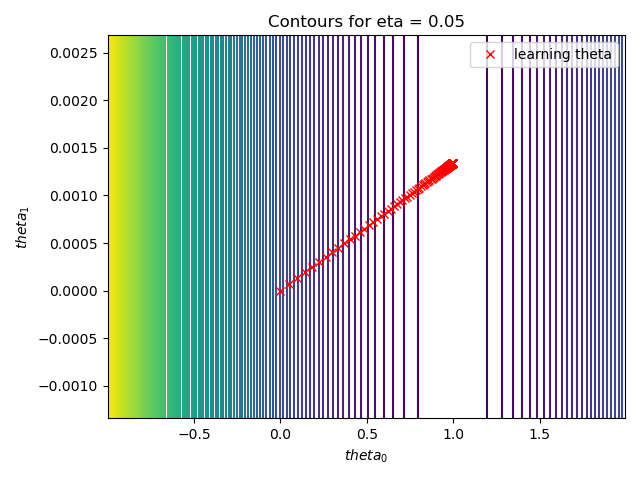
\includegraphics[width=0.7\textwidth]{Q1/output/d.png}
    \caption{Movement of $\theta$ over the Contours}
\end{figure}

\subsection{Experimenting with Different $\eta$}
\begin{figure}[H]
    \centering
    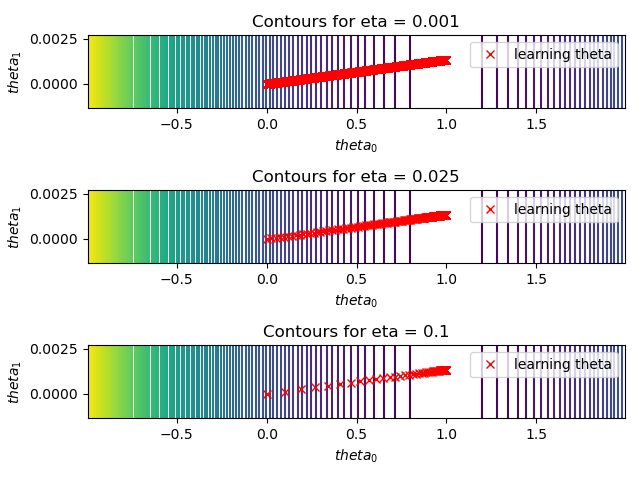
\includegraphics[width=0.7\textwidth]{Q1/output/e.png}
    \caption{Movement of $\theta$ for different $\eta$}
\end{figure}


\section{Sampling and Stochastic Gradient Descent}

\subsection{Sampling}
The data is sampled as follows:
\begin{equation}
    \begin{split}
        x &\sim
        \begin{pmatrix}
            \mathcal{N}(3, 4)\\
            \mathcal{N}(-1, 4)
        \end{pmatrix}\\
        y &\sim \theta^T x + \mathcal{N}\left(0, \sqrt{2}\right)
    \end{split}
\end{equation}
$1$ million samples are generated using the above sampling criteria.

\subsection{Stochastic Gradient Descent}
The convergence criteria used is:
\begin{equation}
    |\underset{\text{epoch }t+1}{average}(J(\theta^{t+1})) - \underset{\text{epoch }t}{average}(J(\theta^t))| \leq \varepsilon\text{, where }\varepsilon=10^{-5}
\end{equation}
The following parameters are learnt for different batch sizes:
\begin{center}
    \begin{tabular}{c c c c}
        \toprule
        \textbf{Batch size ($r$)} & \textbf{$\theta$} & \textbf{Iterations} & \textbf{Time taken}\\
        \midrule
        \midrule
        $1$ &
        $\begin{pmatrix}
            2.99630\\
            0.98101\\
            1.99178
        \end{pmatrix}$
        & $3000000$ ($3$ epochs) & $43.42$ seconds\\
        \midrule
        $100$ &
        $\begin{pmatrix}
            2.99767\\
            0.99998\\
            1.99899
        \end{pmatrix}$
        & $40000$ ($4$ epochs) & $0.74$ seconds\\
        \midrule
        $10000$ &
        $\begin{pmatrix}
            2.96458\\
            1.00759\\
            1.99770
        \end{pmatrix}$
        & $16200$ ($162$ epochs) & $4.29$ seconds\\
        \midrule
        $1000000$ &
        $\begin{pmatrix}
            2.64004\\
            1.07834\\
            1.97405
        \end{pmatrix}$
        & $7535$ ($7535$ epochs) & $105.58$ seconds\\
        \bottomrule
    \end{tabular}
\end{center}

\subsection{Test Error}\label{2c}
The errors for different batch sizes on the test set are:
\begin{center}
    \begin{tabular}{c c}
        \toprule
        \textbf{Batch size ($r$)} & \textbf{Error}\\
        \midrule
        $1$ & $1.00680$\\
        $100$ & $0.98315$\\
        $10000$ & $0.98645$\\
        $1000000$ & $1.35444$\\
        \midrule
        \textit{original $\theta$} & $0.98295$\\
        \bottomrule
    \end{tabular}
\end{center}
The different algorithms (as a parameter of the batch size) have different converging values of $\theta$ and thus different values of test error too. The best predictions are done by the algorithms with batch sizes $100$ and $10000$. Both of them reach convergence in a very small time but taking different number of iterations.\par
Convergence is the fastest for smaller batch sizes which are not too small. This is because computation of the smaller batches is much quicker than larger batches. However, it needs to be noted that the drawback of having a very small batch size is that the data isn't representative enough for the entire sample and hence $\theta$ doesn't converge perpendicular to the contours but instead moves at an angle to it. This slows down the convergence and hence having a slightly larger batch size
(which is still relatively small) is ideal.\par
For larger batch sizes, the jump in $\theta$ is relatively larger towards the best value, however, the computation for each jump is costlier. Additionally, this \textit{direct} jump leads to early convergence since the change in $\theta$ reduces as we reach closer to the optimal value. This leads to smaller change in the cost function since the contours are farther spaced as we approach closer to the optimal value. Thus, we need a smaller $\varepsilon$ for larger batch sizes to converge to the same value.

\subsection{Movement of $\theta$ in the $\theta$ Space}
\begin{figure}[H]
    \begin{subfigure}[t]{0.45\textwidth}
        \centering
        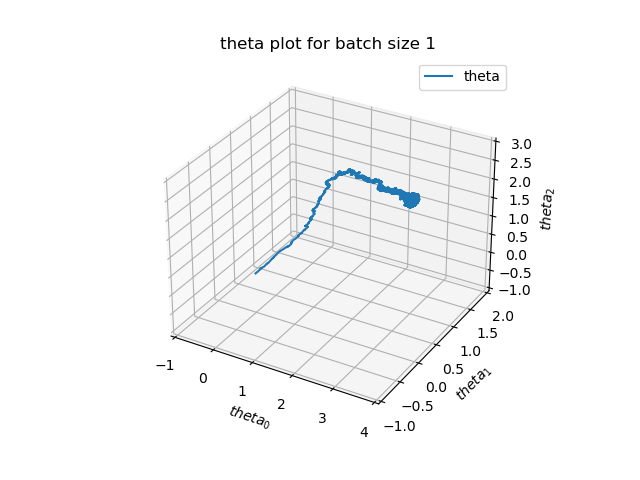
\includegraphics[width=\linewidth]{Q2/output/d1.png}
        \caption{$r=1$}
    \end{subfigure} 
    \hfill
    \begin{subfigure}[t]{0.45\textwidth}
        \centering
        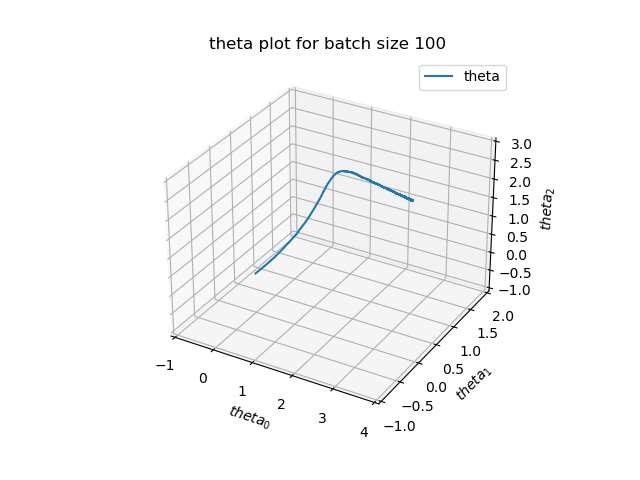
\includegraphics[width=\linewidth]{Q2/output/d100.png}
        \caption{$r=100$}
    \end{subfigure} 
    \medskip
    \begin{subfigure}[t]{0.45\textwidth}
        \centering
        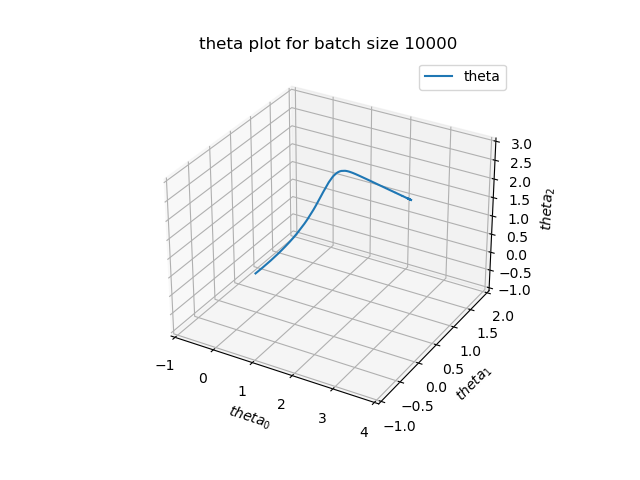
\includegraphics[width=\linewidth]{Q2/output/d10000.png}
        \caption{$r=10000$}
    \end{subfigure}
    \hfill
    \begin{subfigure}[t]{0.45\textwidth}
        \centering
        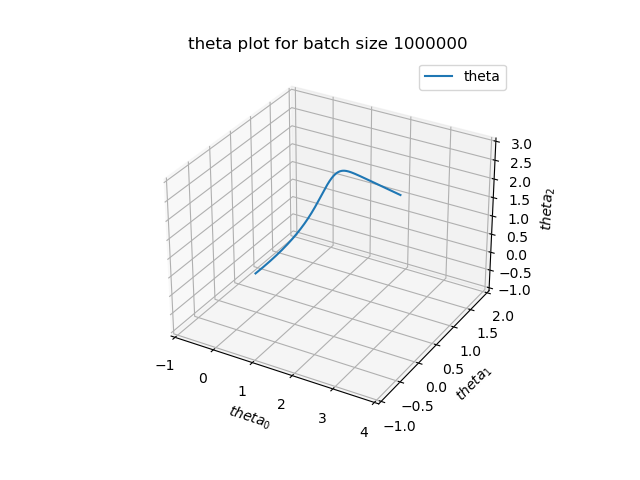
\includegraphics[width=\linewidth]{Q2/output/d1000000.png}
        \caption{$r=1000000$}
    \end{subfigure} 
    \caption{Movement of $\theta$ for different batch sizes}
\end{figure}

The movement of $\theta$ in each of the $4$ cases above is consistent with the explanation given in Section~\ref{2c}. When $r=1$, $\theta$ fluctuates a lot closer to the minimal value and hence convergence is slowed down. Movement of $\theta$ for $r=100, 10000$ is relatively smoother and thus convergence is reached in a small time. For the case of $\theta=1000000$, convergence criteria is met much before $\theta$ reaches close to the optimal value. This is because the change in
consecutive values of $\theta$ leads to a smaller change in the cost function since the contours are not as close when closer to the optimal value.


\section{Logistic Regression}

\subsection{Newton's Method}
To compute the equation of the separator using \textit{Newton's method}, we need to compute the double derivative of $LL(\theta)$, i.e., the \textit{Hessian matrix}. We proceed as follows:
\begin{equation}
    \begin{split}
        \mathcal{H}(LL(\theta)) &= \frac{\partial\left(\nabla_\theta(LL(\theta))\right)}{\partial\theta}\\
        &= \frac{\partial}{\partial\theta}{\left(X^T\left(Y - \frac{1}{1+e^{-X\theta}}\right)\right)}^T\\
        &=
        \begin{pmatrix}
            \frac{\partial}{\partial\theta_0}{\left(X^T\left(Y - \frac{1}{1+e^{-X\theta}}\right)\right)}^T\\
            \frac{\partial}{\partial\theta_1}{\left(X^T\left(Y - \frac{1}{1+e^{-X\theta}}\right)\right)}^T\\
            \vdots\\
            \frac{\partial}{\partial\theta_n}{\left(X^T\left(Y - \frac{1}{1+e^{-X\theta}}\right)\right)}^T
        \end{pmatrix}\\
    \end{split}
\end{equation}
Now, computing each row separately, we get:
\begin{equation}
    \begin{split}
        \mathcal{H}_i &= \frac{\partial}{\partial\theta_i}{\left(X^T\left(Y - \frac{1}{1+e^{-X\theta}}\right)\right)}^T\\
        &= \frac{\partial}{\partial\theta_i}\left(\left(\frac{1}{1+e^{-X\theta}}\right)^T X\right)\\ % chktex 3
        &= \frac{\partial(X\theta)^T}{\partial\theta_i}\frac{\partial\left(\frac{1}{1+e^{-X\theta}}\right)^T}{\partial(X\theta)^T} X\\ % chktex 3
        &= X_i^T \left(\frac{e^{-(X\theta)^T}}{\left(1+e^{-(X\theta)^T}\right)^2}\right) X % chktex 3
    \end{split}
\end{equation}
The complete \textit{Hessian matrix} can thus be written as:
\begin{equation}
    \mathcal{H} = X^T I_m \left(\frac{e^{-(X\theta)^T}}{\left(1+e^{-(X\theta)^T}\right)^2}\right) X\text{, where }I_m=\text{identity matrix} % chktex 3
\end{equation}
We can now perform iterations as follows:
\begin{equation}
    \theta^{t+1}\gets\theta^t-\mathcal{H}^{-1}\nabla_\theta(LL(\theta))
\end{equation}
On learning the model using \textit{Newton's method}, we get the following $\theta$ in $9$ iterations when $\varepsilon$ is $10^{-20}$:
\begin{equation}
    \theta =
    \begin{pmatrix}
        0.40125\\
        2.58855\\
        -2.72559
    \end{pmatrix}
\end{equation}

\subsection{Regression Plot}
\begin{figure}[H]
    \centering
    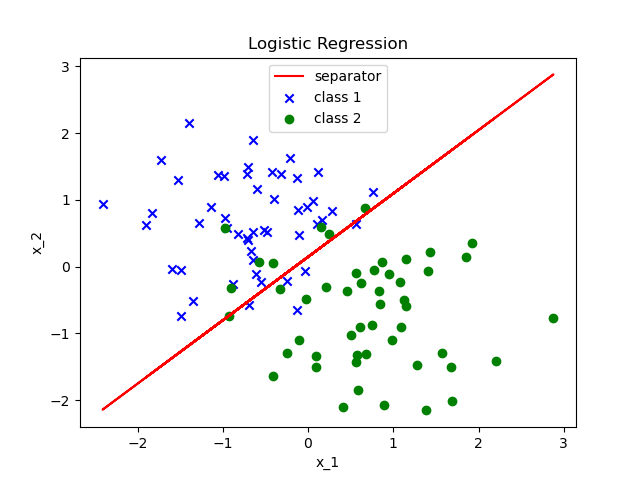
\includegraphics[width=0.7\textwidth]{Q3/output/b.png}
    \caption{Plot of the data along with the separator}
\end{figure}


\section{Gaussian Discriminant Analysis}

\subsection{Linear GDA}
Classifying Alaska as $1$ and Canada as $0$, the model ($\Theta$) for \textit{linear GDA} is obtained as follows:
\begin{equation}
    \begin{split}
        \phi &= 0.5\\
        \mu_0 &=
        \begin{pmatrix}
            0.75529\\
            -0.68509
        \end{pmatrix}\\
        \mu_1 &=
        \begin{pmatrix}
            -0.75529\\
            0.68509
        \end{pmatrix}\\
        \Sigma &=
        \begin{pmatrix}
            0.42953 & -0.02247\\
            -0.02247 & 0.53065
        \end{pmatrix}
    \end{split}
\end{equation}

\subsection{Training Data Plot}
Plot is done in Section~\ref{4e}.

\subsection{Linear Separator Plot}
The separator is given by:
\begin{equation}
    \log\left(\displaystyle\frac{1-\phi}{\phi}\right) - (\mu_1-\mu_0)^T\Sigma^{-1}x + \frac{1}{2}\left(\mu_1^T\Sigma^{1}\mu_1+\mu_0^T\Sigma^{-1}\mu_0\right)=0 % chktex 3
\end{equation}
Plot is done in Section~\ref{4e}.

\subsection{Generic (Quadratic) Separator}
The following parameters ($\Theta$) are obtained for \textit{generic GDA}:
\begin{equation}
    \begin{split}
        \phi &= 0.5\\
        \mu_0 &=
        \begin{pmatrix}
            0.75529\\
            -0.68509
        \end{pmatrix}\\
        \mu_1 &=
        \begin{pmatrix}
            -0.75529\\
            0.68509
        \end{pmatrix}\\
        \Sigma_0 &=
        \begin{pmatrix}
            0.47747 & 0.10992\\
            -0.10992 & 0.41355
        \end{pmatrix}\\
        \Sigma_1 &=
        \begin{pmatrix}
            0.38159 & -0.15487\\
            -0.15487 & 0.64774
        \end{pmatrix}
    \end{split}
\end{equation}

\subsection{Generic Separator Plot}\label{4e}
The separator is given by:
\begin{equation}
    \log\left(\displaystyle\frac{1-\phi}{\phi}\sqrt{\displaystyle\frac{|\Sigma_1|}{|\Sigma_0|}}\right) + \frac{1}{2}\left(x^T(\Sigma_1^{-1}-\Sigma_0^{-1})x - 2(\mu_1^T\Sigma_1^{-1}-\mu_0^T\Sigma_0^{-1})x + \mu_1^T\Sigma_1^{-1}\mu_1 - \mu_0^T\Sigma_0^{-1}\mu_0\right) = 0
\end{equation}
The plot of the data along with the linear and generic separator is:
\begin{figure}[H]
    \centering
    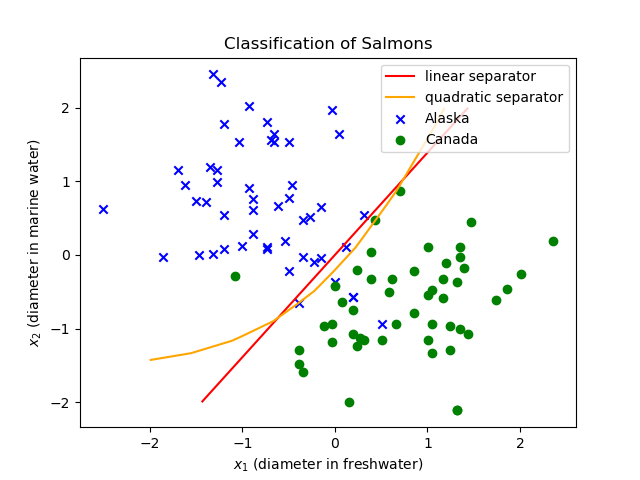
\includegraphics[width=0.7\textwidth]{Q4/output/bce.png}
    \caption{Plot of the data along with the separators}
\end{figure}

\subsection{Analysing the Separators}
The quadratic separator barely fits about two more points correctly compared to the linear separator. Additionally, the quadratic separator gives the notion that we are more \textit{likely} to have salmons from Canada as compared to Alaska since the separator bends towards Alaska. But looking at the training data, it is apparent that it is not the case. Therefore, the quadratic separator leads to overfitting on the test data without actually giving significantly better results even on
the test data.


\end{document}
